\documentclass[aspectratio=169,usenames,dvipsnames]{beamer}
\usepackage{preamble}

\title{Coding for Humanities}
\author{Andreas van Cranenburgh}
\date{Week 7: Tabular data analysis with Pandas}

\begin{document}
\maketitle


\begin{frame}{Last week}
    Exploratory analysis of one variable

    \vspace{1em}
    Visualizations, plots

    \vspace{1em}
    Pandas Series objects
\end{frame}

\begin{frame}{Program for today}
\tableofcontents
\end{frame}



\section{More exploratory data analysis}
\subsection{Exploring two variables}
\frame{\tableofcontents[currentsubsection]}

\begin{frame}{Inspecting two variables}
\begin{description}
    \item[If both categorical:]
            contingency table, bar plot with multiple colors
    \item[One categorical, one continuous:] multi-panel plot.\\
            For each categorical value, plot histogram / boxplot
    \item[Both continuous:]
         scatter plot, look at correlation
\end{description}
\end{frame}

\begin{frame}[fragile]{Two categorical variables}
    \begin{columns}[T]
        \column{0.5\linewidth}
            Contingency table:
            \vspace{1em}

            \begin{tabular}{lrrr}
                & Red & Blue & Yellow \\ \midrule
            men   & 12  & 34 & 56 \\
            women & 21  & 43 & 65 \\
            \end{tabular}

            \vspace{1em}
            Table: favorite colors.
        \column{0.5\linewidth}
            Bar plot:

            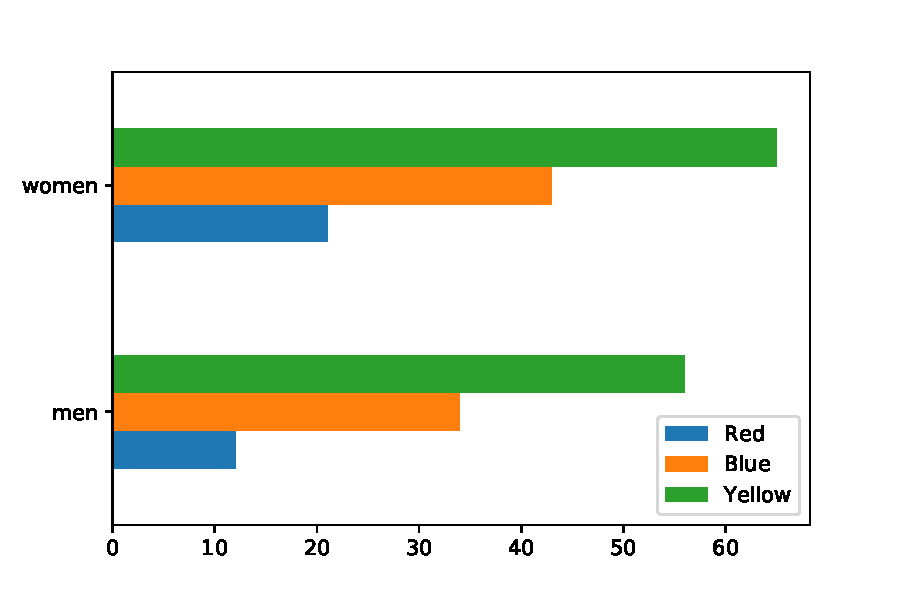
\includegraphics[width=\linewidth]{fig/barcatcont}
    \end{columns}
\begin{lstlisting}
df = pd.DataFrame(
        {'Red': [12, 21], 'Blue': [34, 43], 'Yellow': [56, 65]},
        index=['men', 'women'])
df.plot.barh()
\end{lstlisting}
\end{frame}


\begin{frame}[fragile]{One categorical, one continuous variable}
    \begin{columns}[T]
        \column{0.45\linewidth}
            Histograms:

            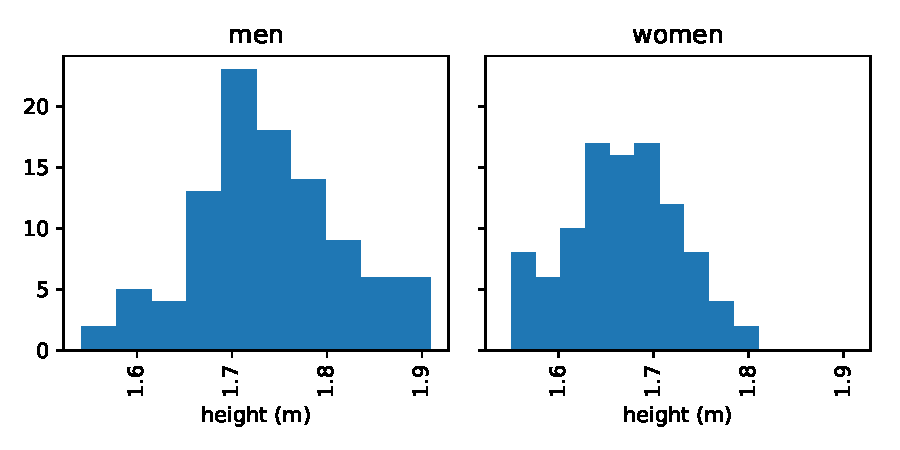
\includegraphics[width=0.9\linewidth]{fig/contcontheighthist}

\begin{lstlisting}
In: df  # tidy data format!
    height   gender
0   1.667763    men
1   1.709885    men
...
\end{lstlisting}
        \column{0.53\linewidth}
            Box plots:

            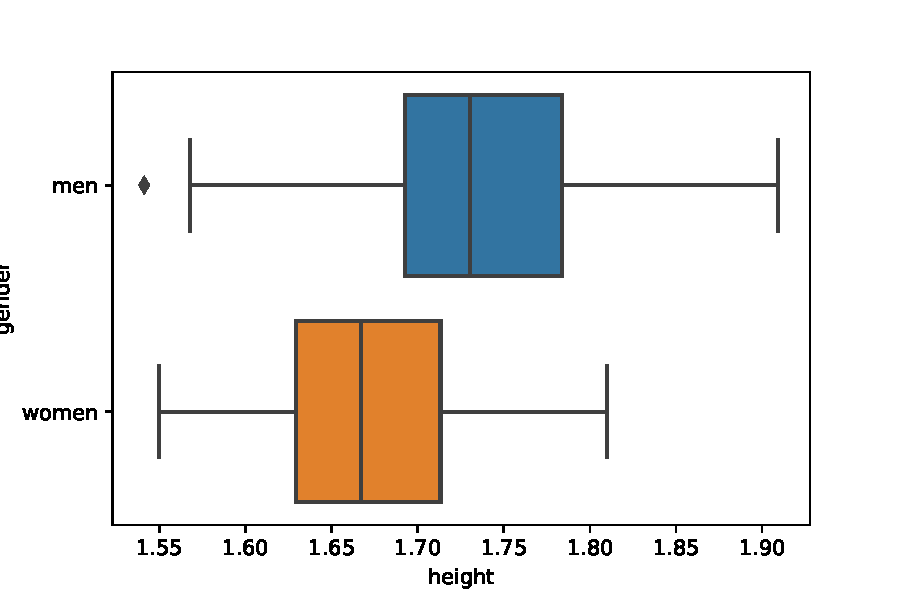
\includegraphics[width=0.9\linewidth]{fig/contcontheightbox}

\begin{lstlisting}
sns.boxplot(x='height', y='gender', data=df)
\end{lstlisting}
    \end{columns}
\begin{lstlisting}
ax = df.hist(by='gender', sharex=True, sharey=True, figsize=(6, 3));
ax[0].set_xlabel('height (m)'); ax[1].set_xlabel('height (m)'); 
\end{lstlisting}
\end{frame}

\begin{frame}{Correlations}
Variables X and Y vary together

\begin{block}{Causality vs.\ correlation:}
Does movement in X ``cause''
movement in Y in some metaphysical sense?
\end{block}

\begin{description}[Correlation]
    \item[Correlation]
        \begin{itemize}
            \item Simultaneous movement through a statistical relationship
            \item Simultaneous variation ``induced'' by the variation of a
                common third effect
        \end{itemize}
    \end{description}
\end{frame}

\begin{frame}{House prices \& per capita income}
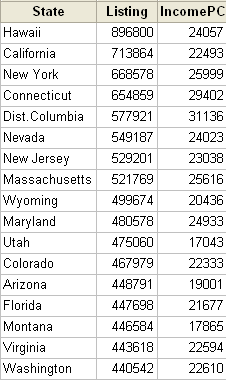
\includegraphics[height=0.85\textheight]{fig/housepricesincome}
\end{frame}

\begin{frame}{Scatter plot suggests positive correlation}
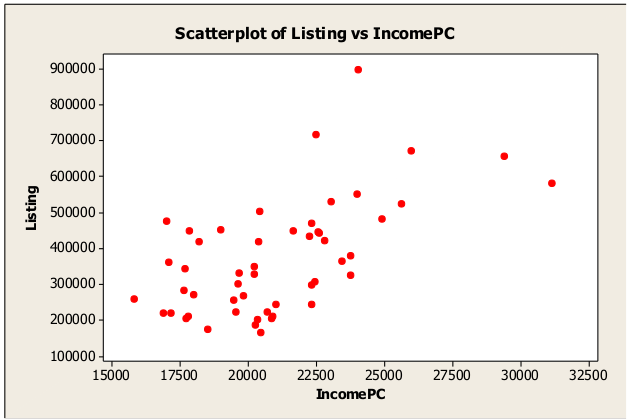
\includegraphics[height=0.7\textheight]{fig/incomelistingscatter}
\end{frame}

\begin{frame}{Correlation is not causation}
Does a rise in income \structure{cause} a rise in gas prices?!

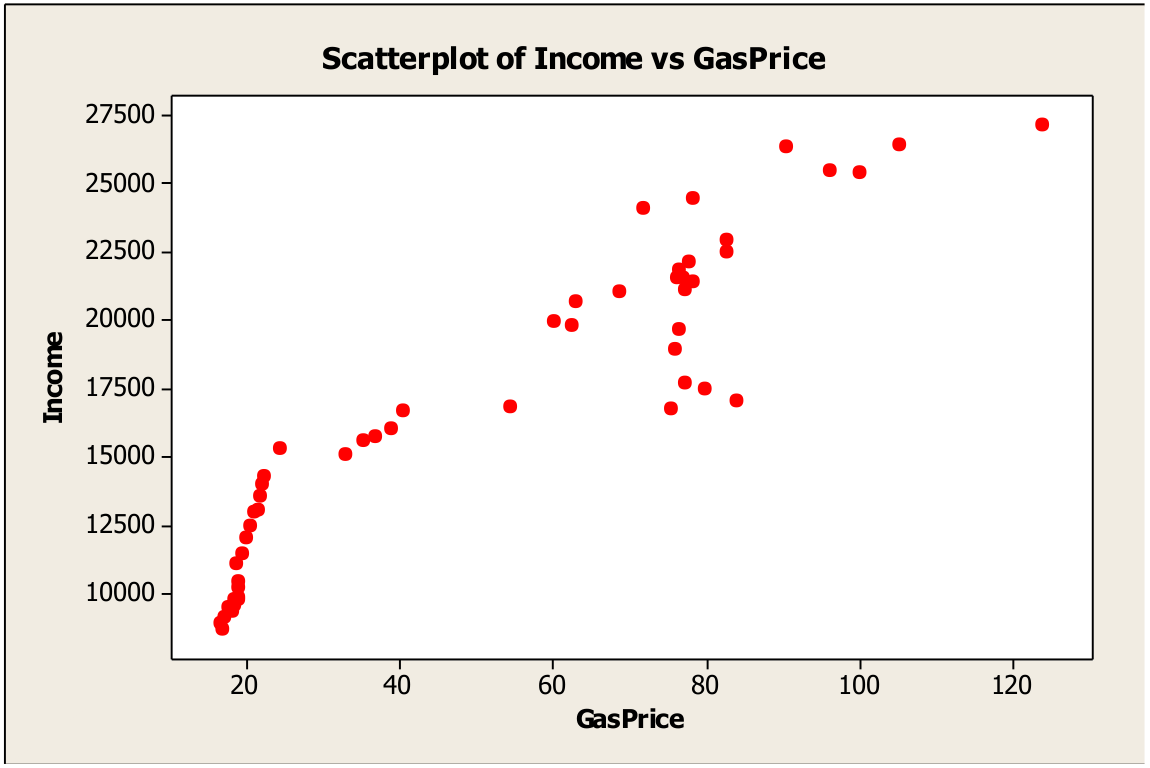
\includegraphics[height=0.7\textheight]{fig/incomegas}

US gasoline prices, 1953-2004, plotted against per-capita US income
\end{frame}

\begin{frame}{Omitted variable: time}
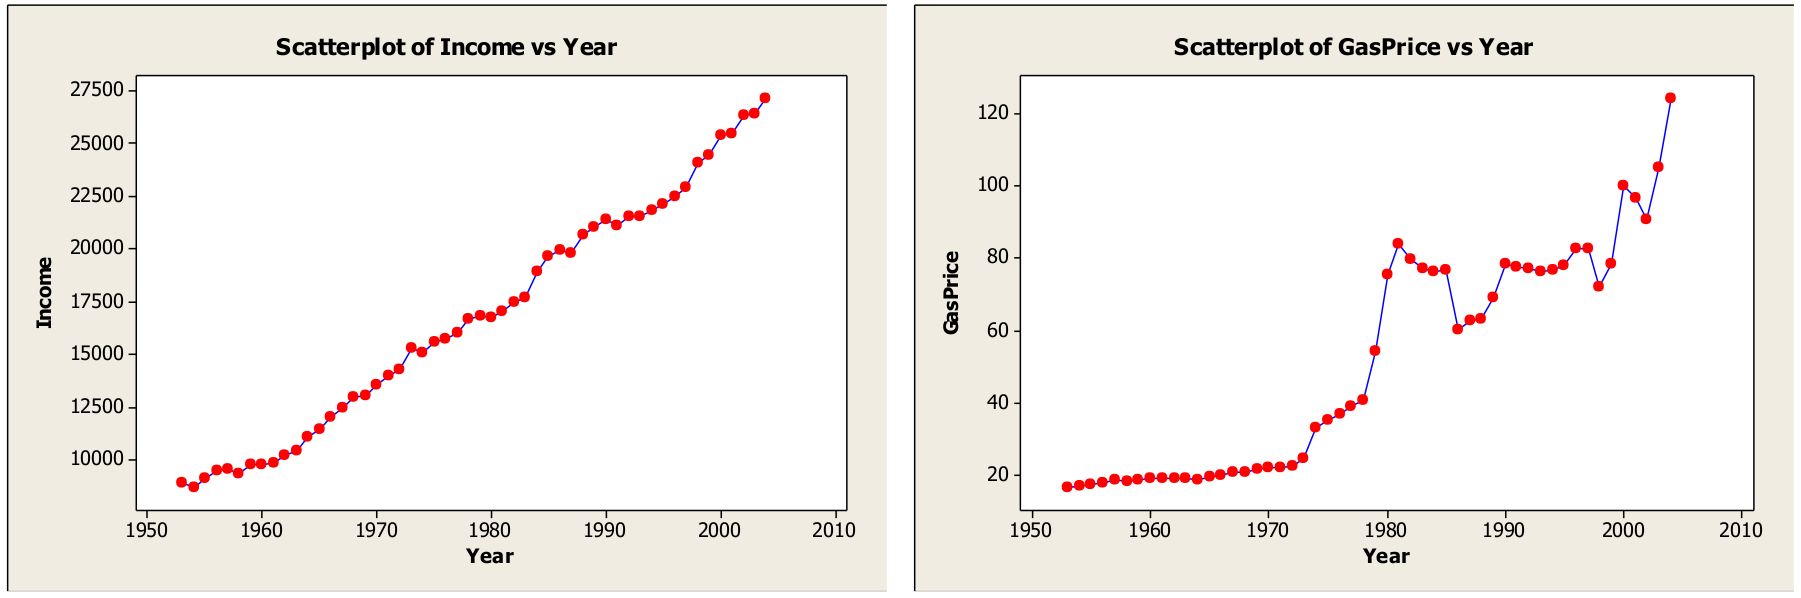
\includegraphics[width=0.99\textwidth]{fig/incomegastime}

No, both income and gas price rise with time (confounding factor).
\end{frame}


\begin{frame}{Pearson's correlation coefficient $r$}
Want to capture:
some variable X varies in the same direction
and at the same scale as some other variable Y

\vspace{1em}
Pearson $r$ measures linear association of two variables.

$r$ is \structure{unitless} in [-1, +1]:

\begin{itemize}
    \item -1 perfect inverse/negative correlation
    \item 0 no \structure{linear} relation
    \item 1 perfect positive correlation
\end{itemize}
\end{frame}

\begin{frame}{House price and income}
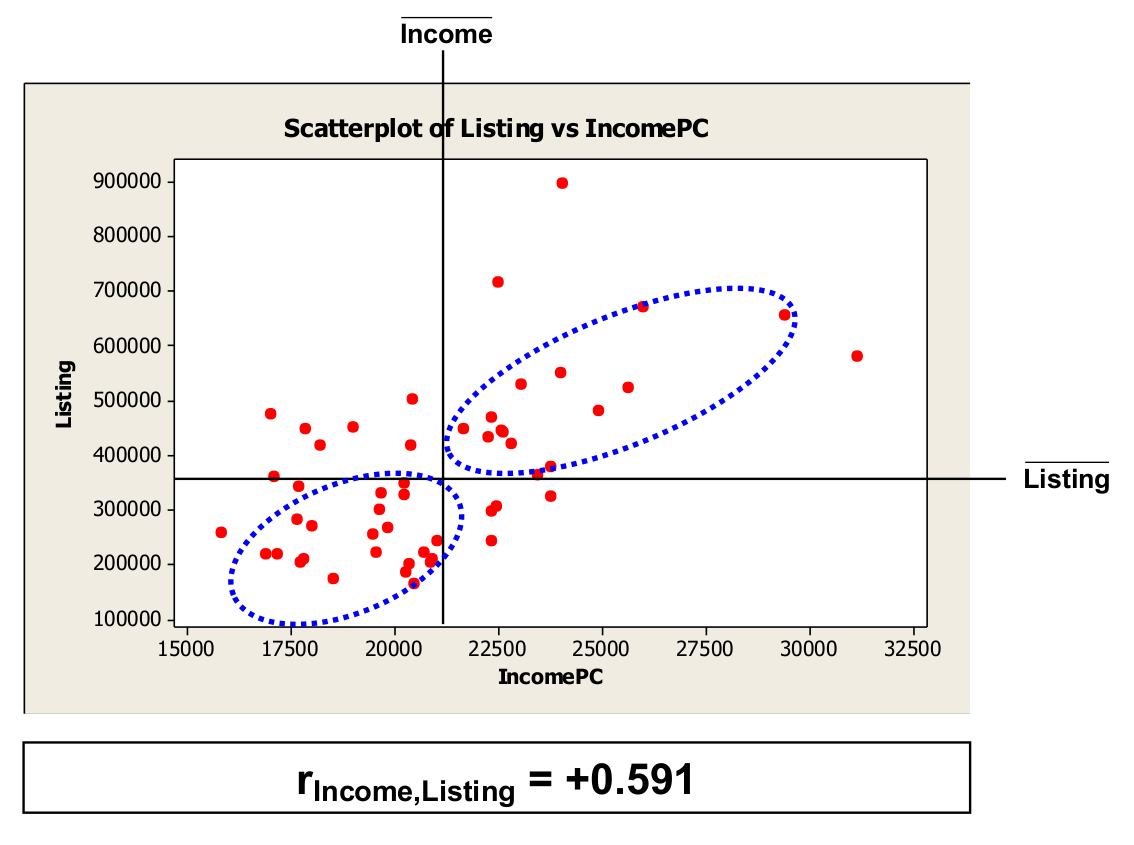
\includegraphics[height=0.8\textheight]{fig/incomelistingcorr}
\end{frame}

\begin{frame}{Examples of $r$}
\begin{reference}\vspace{1em}
Figure: \url{https://en.wikipedia.org/wiki/Correlation_and_dependence}
\end{reference}
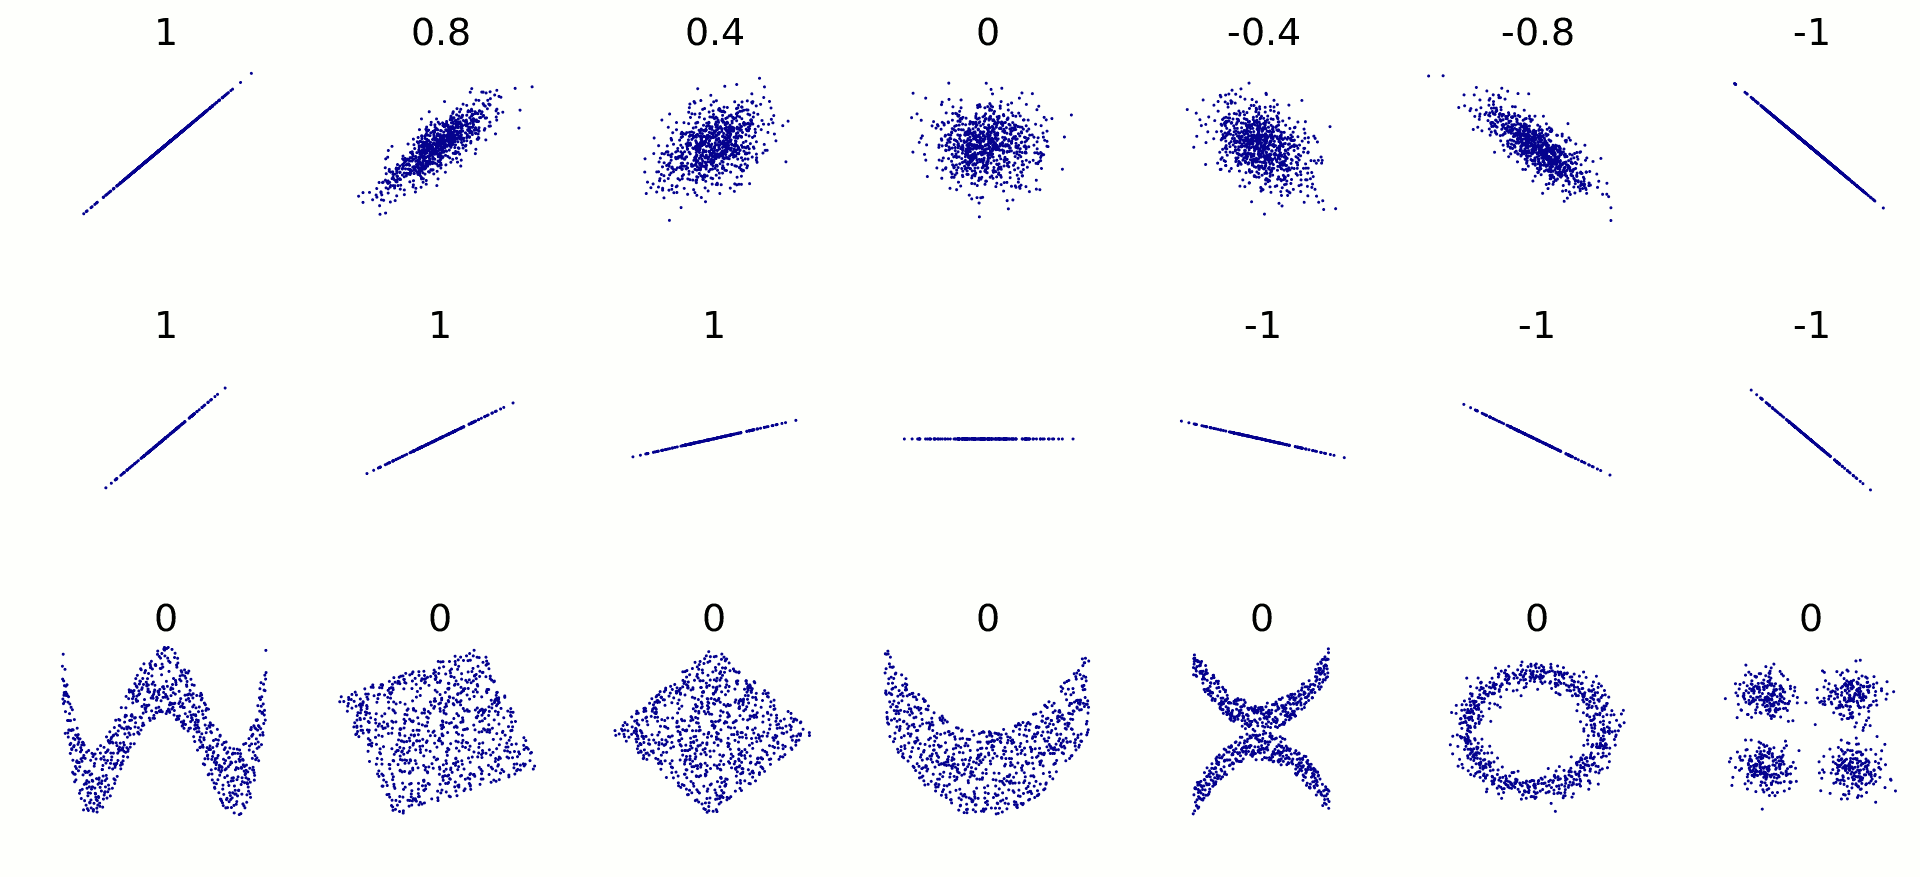
\includegraphics[height=0.6\textheight]{fig/wpcorrelation}

\begin{itemize}
    \item Amount of noise determines strength of correlation
    \item Not slope!
    \item Only linear relationship is measured
\end{itemize}
\end{frame}

\begin{frame}{Correlation is not causation}
\begin{reference}\vspace{1em}
    \url{http://tylervigen.com/spurious-correlations}
\end{reference}
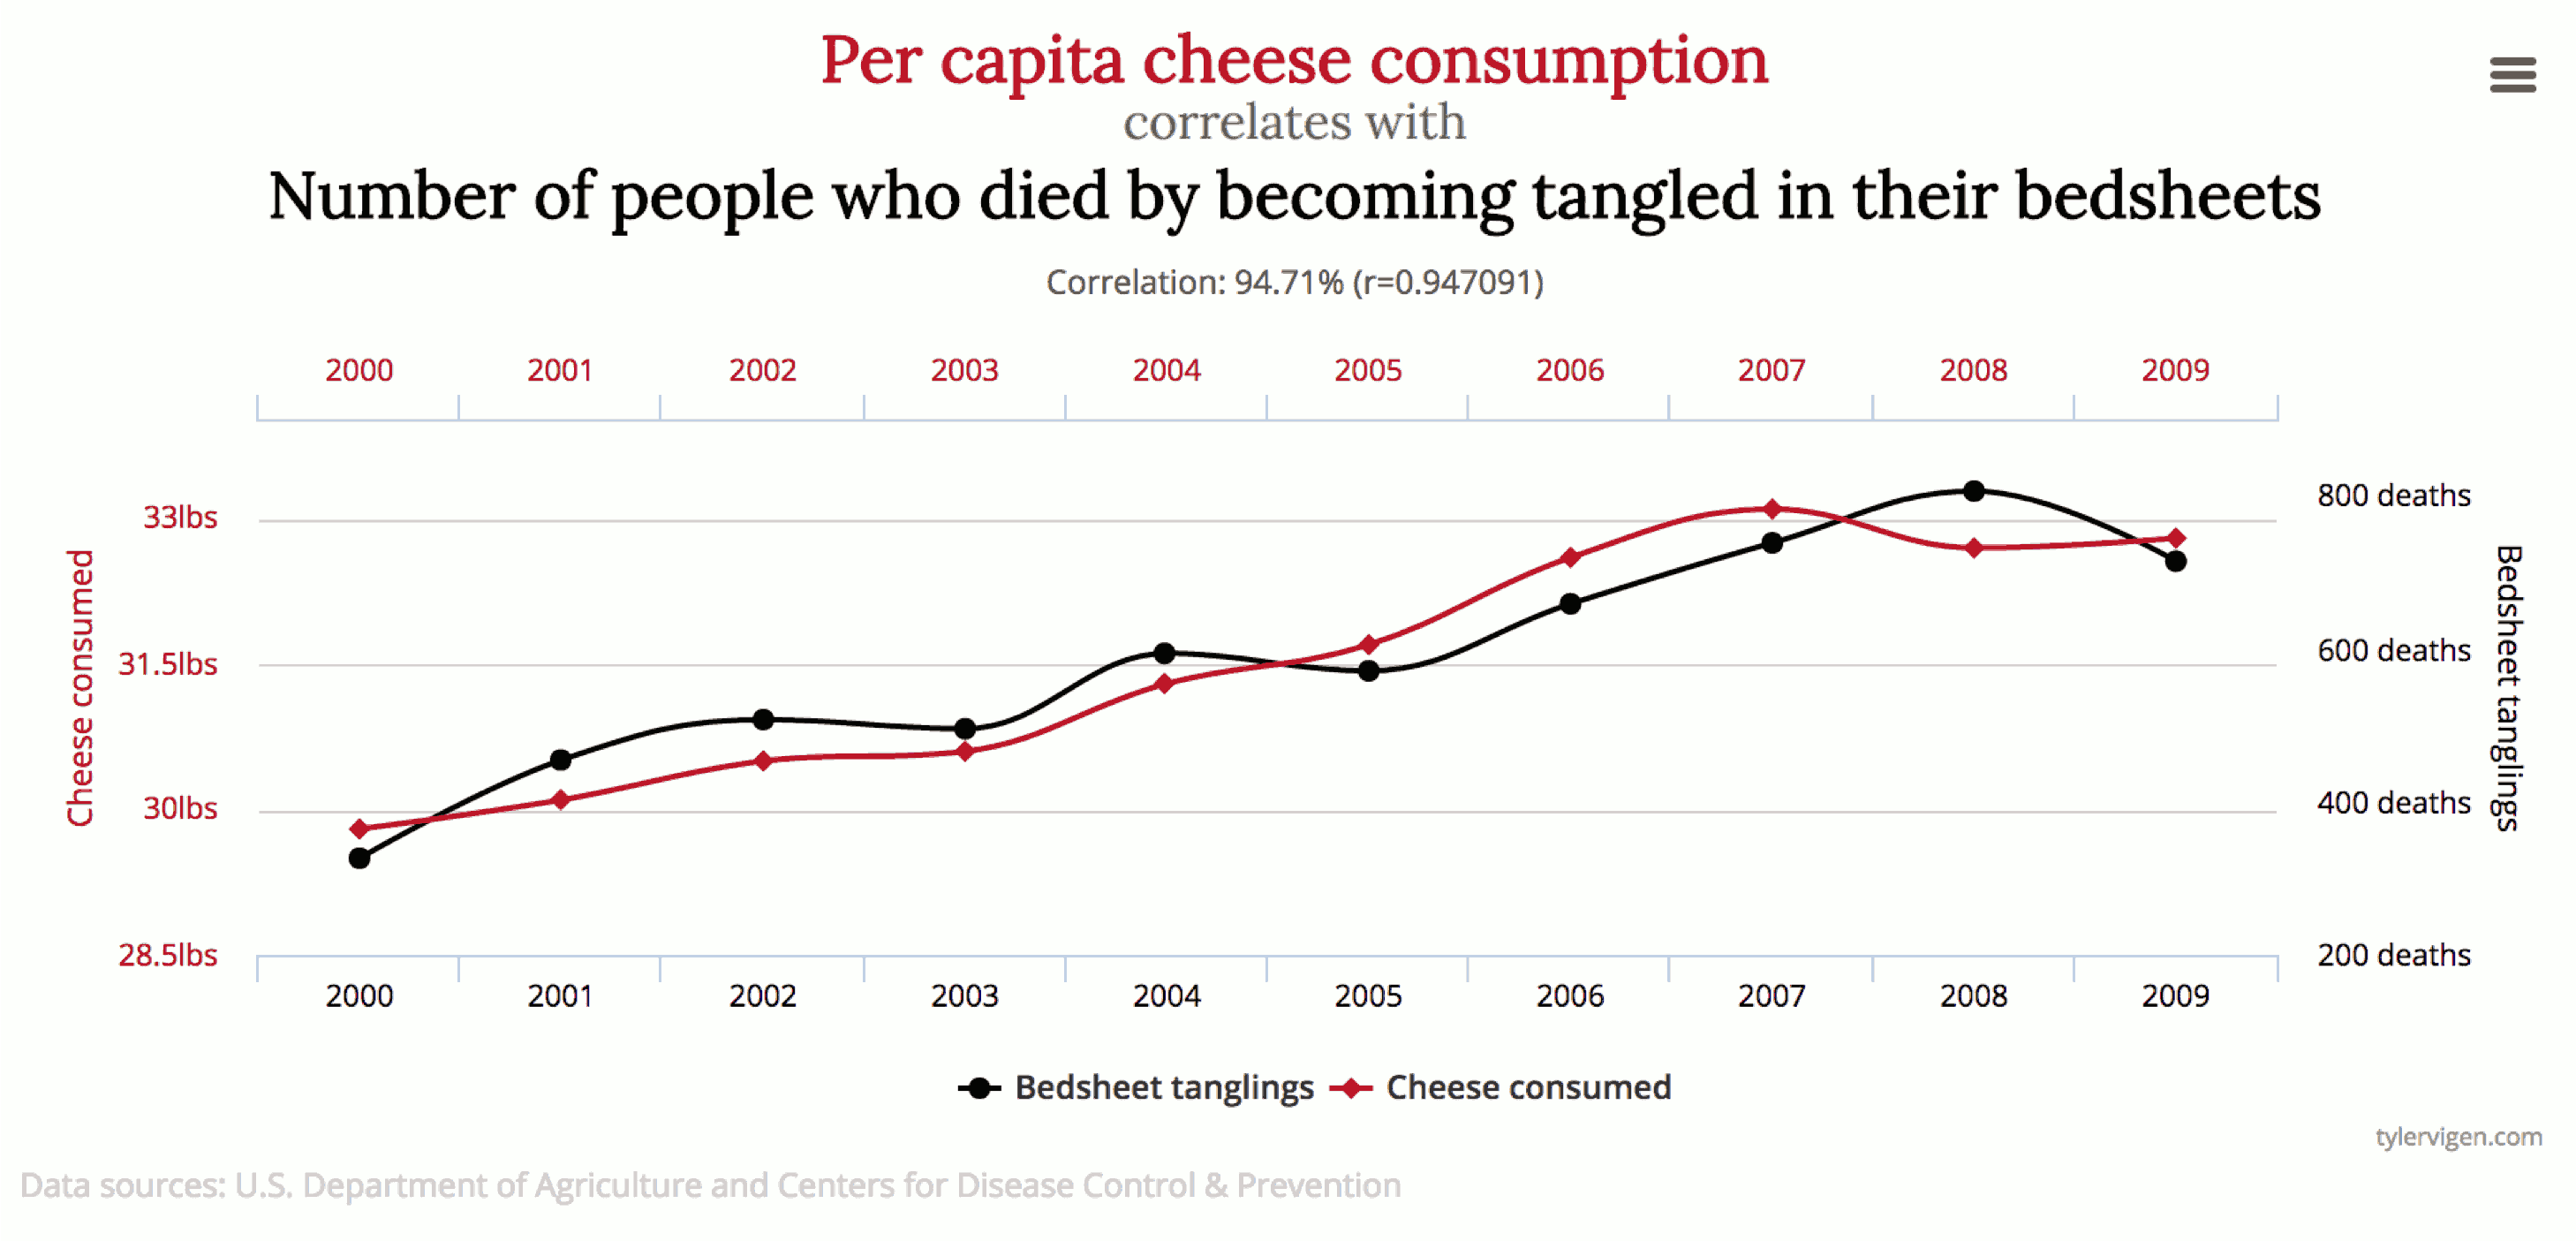
\includegraphics[width=0.99\textwidth]{fig/cheese}
\end{frame}

\begin{frame}{Summary: two variables}
Two \structure{continuous} variables:
\begin{enumerate}
    \item Look at the data! Make a scatter plot
    \item Compute correlation
    \item Think carefully whether the relation is meaningful!
\end{enumerate}
\end{frame}



\section{Exploring tabular datasets with Pandas}
\frame{\tableofcontents[currentsection]}

% From http://swcarpentry.github.io/python-novice-gapminder/
% Reading Tabular Data into DataFrames
%     Use the Pandas library to get basic statistics out of tabular data.
%     Use index_col to specify that a column's values should be used as row headings.
%     Use DataFrame.info to find out more about a dataframe.
%     The DataFrame.columns variable stores information about the dataframe's columns.
%     Use DataFrame.T to transpose a dataframe.
%     Use DataFrame.describe to get summary statistics about data.

% missing: index_col, .T

% Pandas DataFrames
%     Use DataFrame.iloc[..., ...] to select values by integer location.
%     Use : on its own to mean all columns or all rows.
%     Select multiple columns or rows using DataFrame.loc and a named slice.
%     Result of slicing can be used in further operations.
%     Use comparisons to select data based on value.
%     Select values or NaN using a Boolean mask.


% Plotting
%     matplotlib is the most widely used scientific plotting library in Python.
%     Plot data directly from a Pandas dataframe.
%     Select and transform data, then plot it.
%     Many styles of plot are available: see the Python Graph Gallery for more options.
%     Can plot many sets of data together.



%\begin{frame}{Creating a DataFrame}
%\end{frame}

%\begin{frame}{Loading a dataset}
%use pandas.read\_csv()
%%     Use index_col to specify that a column's values should be used as row headings.
% \end{frame}
%\begin{frame}{Basic information}
%     Use DataFrame.info to find out more about a dataframe.
%     The DataFrame.columns variable stores information about the dataframe's columns.
%\end{frame}

%     Use DataFrame.T to transpose a dataframe.
%     Use DataFrame.describe to get summary statistics about data.
















\begin{frame}[fragile]{Reading files}
A Comma-Separate Value (CSV) file \texttt{example.csv}:

\begin{lstlisting}[style=plain]
Name,Length,Favorite_Color
John,1.77,Black
Mary,1.66,Blue
[...]
\end{lstlisting}

Reading a CSV-file:
\begin{lstlisting}
>>> import pandas as pd
>>> df = pd.read_csv('example.csv')
\end{lstlisting}

Or: \texttt{pd.read\_excel()}
\end{frame}

\begin{frame}[fragile]{The index column}
To use the first column (0) as index:
\begin{lstlisting}
>>> df = pd.read_csv('example.csv', index_col=0)
\end{lstlisting}

Can also specify the name of a column in the file:

\begin{lstlisting}
>>> df = pd.read_csv('example.csv', index_col='Name')
\end{lstlisting}

\pause
    \begin{definition}
        A named \structure{keyword} argument may be given \\
        after required positional arguments.
    \end{definition}
\end{frame}

\begin{frame}[fragile]{Writing data}
Writing to a csv file.

\begin{lstlisting}
>>> df.to_csv('foo.csv')
\end{lstlisting}
Or \texttt{df.to\_excel()}
\end{frame}

%\begin{frame}[fragile]{Flipping the tables}
%To flip rows and columns:
%\begin{lstlisting}
%>>> df = df.T
%\end{lstlisting}
%(T for transpose)
%\end{frame}


% Start long tutorial on telecom data
\subsection{Analyzing the Telecom dataset}
\begin{frame}{The Telecom dataset}
    Rest of this section:
    \begin{itemize}
        \item Telecom dataset: why do we lose customers?
        \item Step-by-step walk-through of exploratory analysis.
    \end{itemize}

    \vspace{1em}
    Example courtesy of \url{https://mlcourse.ai/}
\end{frame}

\begin{frame}[fragile]{Reading the telecom data}
\begin{lstlisting}
>>> df = pd.read_csv('telecom_churn.csv')
>>> df.head()
\end{lstlisting}

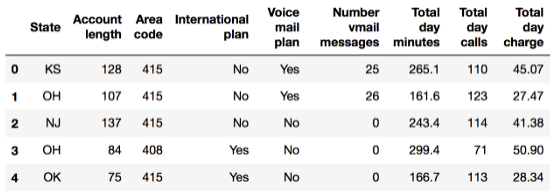
\includegraphics[width=0.9\linewidth]{fig/telecom}

\end{frame}

\begin{frame}[fragile]{Inspecting the shape and columns}
\begin{lstlisting}
>>> df.shape
(3333, 20)
\end{lstlisting}

3333 rows, 20 columns

\begin{lstlisting}
>>> df.columns
Index(['State', 'Account length', 'Area code', 'International plan', ...])
\end{lstlisting}
\end{frame}

\begin{frame}[fragile]{More information}
\begin{columns}
\column{0.65\textwidth}
\begin{lstlisting}
>>> df.info()
<class 'pandas.core.frame.DataFrame'>
RangeIndex: 3333 entries, 0 to 3332
Data columns (total 20 columns):
State                     3333 non-null object
Account length            3333 non-null int64
Area code                 3333 non-null int64
International plan        3333 non-null object
Voice mail plan           3333 non-null object
Number vmail messages     3333 non-null int64
...
Total intl charge         3333 non-null float64
Customer service calls    3333 non-null int64
Churn                     3333 non-null bool
dtypes: bool(1), float64(8), int64(8), object(3)
memory usage: 498.1+ KB
\end{lstlisting}
\column{0.35\textwidth}
    \begin{itemize}
        \item Datatypes:
        \begin{itemize}\item boolean, \item integer, \item floating point, \item and object (strings)\end{itemize}
        \item No missing values (good)
    \end{itemize}
\end{columns}
\end{frame}

\begin{frame}[fragile]{Summary statistics}
    \begin{lstlisting}
    >>> df.describe()
    \end{lstlisting}

    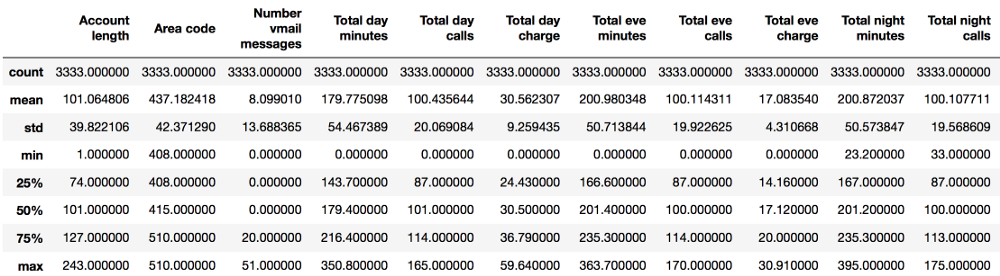
\includegraphics[height=0.5\textheight]{fig/telecomdescribe}
\end{frame}

\begin{frame}[fragile]{Selecting a column}
\begin{lstlisting}
>>> df['Churn']
0       False
1       False
2       False
3       False
4       False
5       False
6       False
...
3330    False
3331    False
3332    False
Name: Churn, Length: 3333, dtype: bool
\end{lstlisting}

This column describes whether a client left or not.
\end{frame}


\begin{frame}[fragile]{Distribution of values}
    \begin{lstlisting}
    >>> df['Churn'].value_counts()
    False    2850
    True      483
    Name: Churn, dtype: bool
    \end{lstlisting}

    2850 clients out of 3333 are loyal

    \vspace{1em}\pause
    Calculate proportion:
    \begin{lstlisting}
    >>> df['Churn'].value_counts(normalize=True)
    False    0.855086
    True     0.144914
    Name: Churn, dtype: float64
    \end{lstlisting}

    14\% churn, very bad!

    \vspace{1em}
    Why are we losing customers?

\end{frame}

\begin{frame}[fragile]{Sorting by a column}
\begin{lstlisting}
>>> df.sort_values(by='Total day charge', ascending=False).head()
\end{lstlisting}

    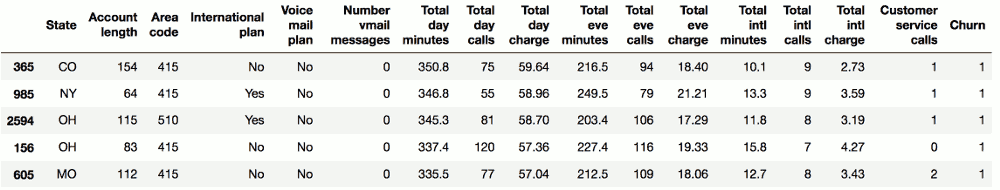
\includegraphics[height=0.3\textheight]{fig/telecomsort}

    ascending=False: from high to low
\end{frame}

\begin{frame}[fragile]{Selecting slices}
    \begin{itemize}
        \item Indexing rows/columns by label:
\begin{lstlisting}
>>> df.loc[0:5, 'State':'Area code']
\end{lstlisting}

            NB: last element is included!

        \item Indexing rows/columns by integer location:

\begin{lstlisting}
>>> df.iloc[0:5, 0:3]
\end{lstlisting}

            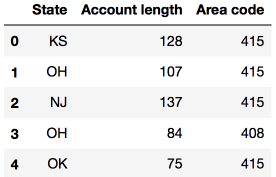
\includegraphics[height=0.3\textheight]{fig/telecomslice}
    \end{itemize}
\end{frame}

\begin{frame}[fragile]{Boolean operations}
Which rows are clients on the international plan?

\begin{lstlisting}
>>> df['International plan'] == 'Yes'
0       False
1       False
2       False
3        True
4        True
5        True
6       False
7        True
8       False
...
3331     True
3332    False
Name: International plan, Length: 3333, dtype: bool
\end{lstlisting}
\end{frame}

\begin{frame}[fragile]{Selecting particular rows}
\begin{lstlisting}
>>> df.loc[df['International plan'] == 'Yes', :]
   State  Account length  Area code International plan \
3     OH              84        408                Yes
4     OK              75        415                Yes
5     AL             118        510                Yes
7     MO             147        415                Yes
9     WV             141        415                Yes
38    AK             136        415                Yes
...
323 rows  x 20 columns
\end{lstlisting}
\end{frame}

\begin{frame}[fragile]{What are the averages for those clients?}
\vspace{-0.5em}
\begin{lstlisting}
>>> df.loc[df['International plan'] == 'Yes', :].mean()
Account length            104.071207
Area code                 443.461300
Number vmail messages       8.464396
Total day minutes         187.986997
Total day calls           100.665635
Total day charge           31.958390
Total eve minutes         203.936842
Total eve calls           100.486068
Total eve charge           17.334923
Total night minutes       196.410217
Total night calls         100.851393
Total night charge          8.838483
Total intl minutes         10.628173
Total intl calls            4.609907
Total intl charge           2.869907
Customer service calls      1.464396
Churn                       0.424149
\end{lstlisting}
\end{frame}

\begin{frame}[fragile]{Answering specific questions}
How much time (on average) do churned clients spend on the phone during daytime?

\begin{lstlisting}
>>> df.loc[df['Churn'] == 1, 'Total day minutes'].mean()
206.91407867494814
\end{lstlisting}

\pause
What is the maximum length of international calls among loyal clients
(Churn == 0) who do not have an international plan?

\begin{lstlisting}
>>> df.loc[
        (df['Churn'] == 0) & (df['International plan'] == 'No'),
        'Total intl minutes'].max()
18.899999999999999
\end{lstlisting}
\end{frame}


% NB: We avoid lambda / higher-order functions!

% \begin{frame}[fragile]{Applying functions to cells, columns, rows}
% \begin{itemize}
%     \item Apply function to each column:
% 
% \begin{lstlisting}
% >>> df.apply(lambda col: col.max())
% 
% State                        WY
% Account length              243
% Area code                   510
% International plan          Yes
% Voice mail plan             Yes
% [...]
% Churn                         1
% dtype: object
% \end{lstlisting}
% 
% \item Apply function to each row: \\
%     \texttt{df.apply(lambda row: row.max(), axis=1)}
% \end{frame}
 
\begin{frame}[fragile]{Renaming things}
Renaming columns / index labels:
\begin{lstlisting}
>>> df = df.rename(columns={'one': 'foo', 'two': 'bar'})
>>> df = df.rename(index={'a': 'apple', 'b': 'banana', 'd': 'durian'})
\end{lstlisting}

Replace values in the \texttt{Voice mail plan} column with proper Boolean values:
\begin{lstlisting}
>>> d = {'No' : False, 'Yes' : True}
>>> df = df.replace({'Voice mail plan': d})
\end{lstlisting}

\end{frame}


\begin{frame}[fragile]{Grouping data}
Recipe:
\begin{lstlisting}
>>> df.groupby(by=grouping_columns)[columns_to_show].function()
\end{lstlisting}

\begin{enumerate}
\item First, collect all values in columns specified
    in \texttt{grouping\_columns}. \\
    These will form the rows in the result.
\item Then, select columns of interest (\texttt{columns\_to\_show}). \\
    If not given, return all other columns.
\item Finally, apply a function to aggregate the data for each group;
    e.g. \texttt{min(), max(), mean()}.
\end{enumerate}
\end{frame}


\begin{frame}[fragile]{Grouping example}
\begin{lstlisting}
>>> columns_to_show = ['Total day minutes', 'Total eve minutes']
>>> df.groupby(['Churn'])[columns_to_show].mean()
      Total day minutes  Total eve minutes
Churn
False           175.175            199.043
True            206.914            212.410
\end{lstlisting}
\end{frame}

\begin{frame}[fragile]{Contingency table}
Count clients across two variables:
\begin{lstlisting}
>>> pd.crosstab(df['Churn'], df['International plan'])
International plan  False  True
Churn
False                2664    186
True                  346    137
\end{lstlisting}
\pause
\begin{lstlisting}
>>> pd.crosstab(df['Churn'], df['Voice mail plan'], normalize=True)
Voice mail plan     False     True
Churn
False            0.602460  0.252625
True             0.120912  0.024002
\end{lstlisting}

Most clients are loyal, do not use extra plans.
\end{frame}

\begin{frame}[fragile]{Adding columns}
Add a new column based on other columns:
\begin{lstlisting}
>>> df['Total charge'] = (df['Total day charge']
        + df['Total eve charge']
        + df['Total night charge']
        + df['Total intl charge'])
>>> df.head()
\end{lstlisting}

Delete rows / columns:

\begin{lstlisting}
>>> # get rid of just created column
>>> df = df.drop(['Total charge'], axis=1)
>>> # and here's how you can delete rows
>>> df.drop([1, 2]).head()
\end{lstlisting}
\end{frame}

\begin{frame}[fragile]{Predicting churn}
\begin{lstlisting}
>>> pd.crosstab(df['Churn'], df['International plan'], margins=True)
International plan    No    Yes      All
Churn
False               2664    186     2850
True                 346    137      483
All                 3010    323     3333
\end{lstlisting}
\end{frame}

\begin{frame}[fragile]{Plotting I}
\begin{lstlisting}
%matplotlib inline
import seaborn as sns
sns.countplot(x='International plan', hue='Churn', data=df);
\end{lstlisting}
\begin{columns}
\column{0.7\textwidth}
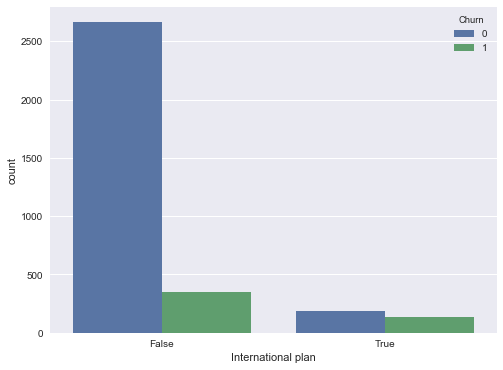
\includegraphics[height=0.6\textheight]{fig/telecomplot}
\column{0.3\textwidth}

With international plan, churn rate is much higher!

\vspace{1em}
Maybe because of large expenses with international calls?
\end{columns}
\end{frame}


\begin{frame}[fragile]{Plotting II}
\begin{lstlisting}
sns.countplot(x='Customer service calls', hue='Churn', data=df);
\end{lstlisting}

\begin{columns}
\column{0.7\textwidth}
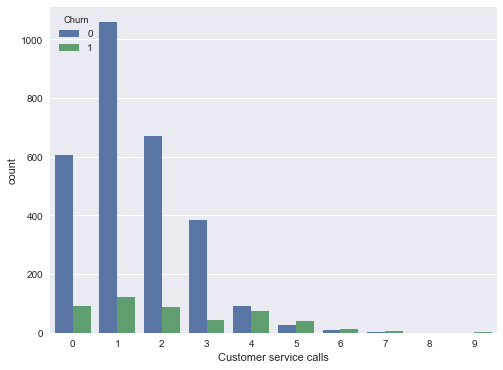
\includegraphics[height=0.6\textheight]{fig/telecomplot2}
\column{0.3\textwidth}
With 4 or more calls, churn rate sharply increases!
\end{columns}
\end{frame}

\begin{frame}[fragile]{Adding a new column}
\begin{lstlisting}
>>> df['Many_service_calls'] = (df['Customer service calls'] > 3)
>>> pd.crosstab(df['Many_service_calls'], df['Churn'], margins=True)
Churn               False  True   All
Many_service_calls
False                2721   345  3066
True                  129   138   267
All                  2850   483  3333
\end{lstlisting}
\end{frame}

\begin{frame}[fragile]{Plotting the new column}
\begin{lstlisting}
>>> sns.countplot(x='Many_service_calls', hue='Churn', data=df);
\end{lstlisting}

\begin{columns}
\column{0.7\textwidth}
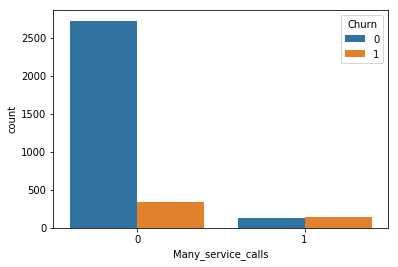
\includegraphics[height=0.6\textheight]{fig/telecomplot3}
\column{0.3\textwidth}
With 4 or more calls, churn rate sharply increases!
\end{columns}
\end{frame}

\begin{frame}[fragile]{Combining two good predictors}
\begin{lstlisting}
>>> pd.crosstab(df['Many_service_calls']
        & df['International plan'],
        df['Churn'])
Churn  False  True
row_0
False   2841    464
True       9     19
\end{lstlisting}
\begin{itemize}
\item These two variables predict the right outcome in \\
    (2841 + 19) / 3333 = 85.8 \% of cases.
\item Slightly better than majority baseline: \\
    2850 / 3333 = 85.5 \%
    (proportion of loyal clients)
\item We can probably do better with advanced methods. \\
    \structure{But}: good to know how well a simple method performs
\end{itemize}
\end{frame}

\begin{frame}[fragile]{Checking a correlation}
\begin{lstlisting}
>>> df['Total day minutes'].corr(df['Total eve minutes'])
0.007042510993777701
>>> sns.jointplot('Total day minutes', 'Total eve minutes', data=df)
\end{lstlisting}

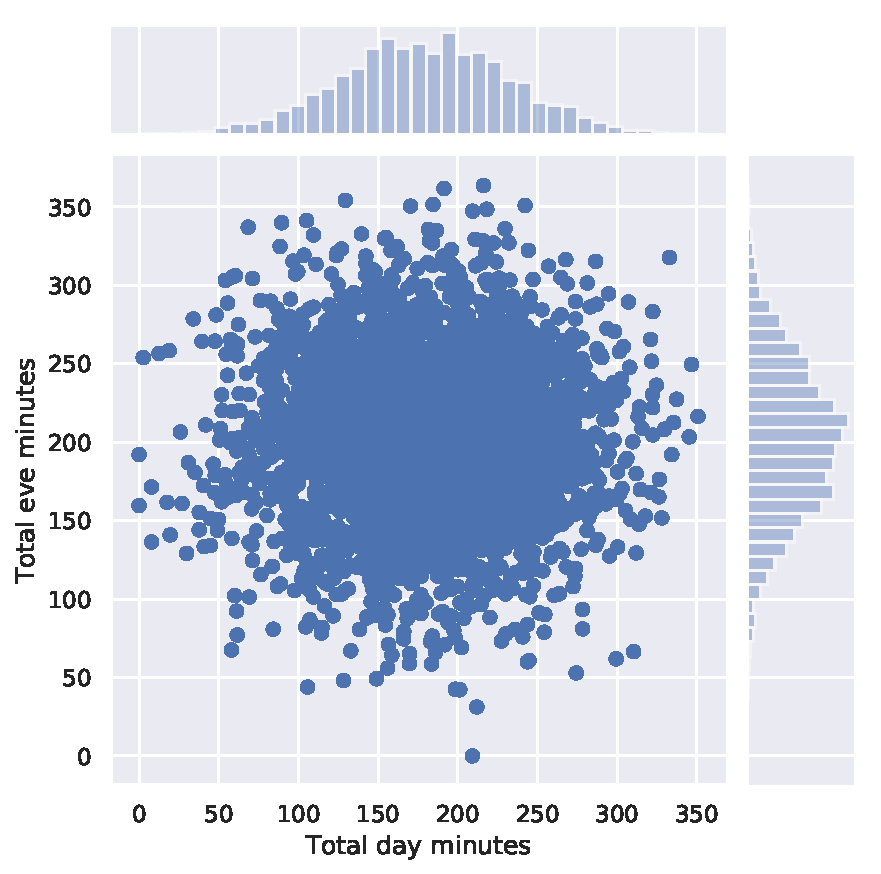
\includegraphics[height=0.6\textheight]{fig/scatter}
\end{frame}

\begin{frame}[fragile]{After exploratory data analysis}
With exploratory data analysis,
we looked at a handful of variables
and created a rule:

\begin{lstlisting}
IF many_service_calls and international_plan
    THEN churn = 1 ELSE churn = 0
\end{lstlisting}

Next steps:
\begin{description}
    \item[Hypothesis testing] Confirm findings with statistical tests
    \item[Machine Learning] Automatically find more patterns:
        \begin{itemize}
            \item Automatically learn many rules
            \item Create more complicated models from thousands of variables
        \end{itemize}
\end{description}
\end{frame}

\section{Course overview}
\frame{\tableofcontents[currentsubsection]}

\begin{frame}{The final exam}
    \begin{itemize}
        \item Study all the slides, notebooks, and exercises of week 1--7
        \item Released Tuesday 15 Oct 2019, 18:00 evening
        \item Due data Monday 28 Oct 2019, 9:00 morning
    \end{itemize}
\end{frame}

\begin{frame}{Learning goals}
    \begin{enumerate}
        \item Write simple programs to perform basic tasks such as searching
            and cleaning text corpora
        \item Work with Jupyter Notebooks and other common Python data science
            tools to report on simple exploratory experiments:
            load a tabular dataset, compute summary statistics,
            and create plots
        \item Understand and solve common errors during programming
        \item Read documentation on available software to evaluate its
            applicability to a problem
        \item Collaborate effectively with programmers using proper terminology
    \end{enumerate}
\end{frame}

\subsection{Where to go from here}
\begin{frame}{Jupyter Notebook}
    \begin{block}{Jupyter Notebook}
        A notebook keeps narrative, code, and results together.

        Ideally, everything can be reproduced with the push of a button.
    \end{block}
    \begin{itemize}
        \item Web-based graphical interface
        \item Mix code, results, and explanation \\
                (Knuth: Literate Programming)
        \item Include plots / pictures
        \item Interactive, rapid prototyping
    \end{itemize}

    \pause
    Pros and cons:
    \begin{itemize}
        \item Why Jupyter is data scientists' computational notebook of choice,
            Nature (2018). \url{https://www.nature.com/articles/d41586-018-07196-1}
        \item Why I don't like notebooks, Joel Grus (2018).
            \url{https://www.youtube.com/watch?v=7jiPeIFXb6U}
    \end{itemize}
\end{frame}

\begin{frame}{Notebook pitfalls}
    \begin{columns}
        \column{0.5\linewidth}
            \begin{itemize}
                \item Hidden state and out-of-order execution:\\
                    Ensure code works by running all cells from start to finish!
                    (Kernel $\rightarrow$ Restart \& Run All)
            \end{itemize}
        \column{0.5\linewidth}
            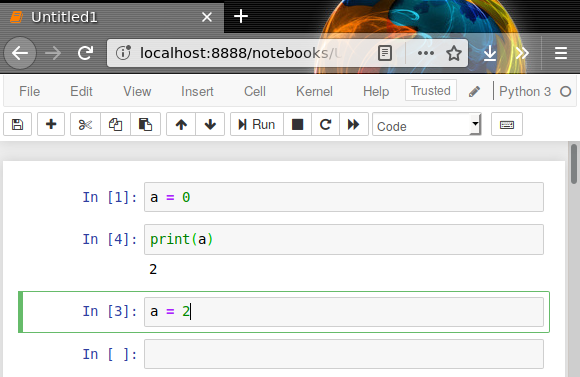
\includegraphics[width=0.95\textwidth]{fig/nboutoforder}
    \end{columns}
    \pause
    \begin{itemize}
        \item Jupyter ``encourages'' throw-away code:\\
                Put re-usable code in a normal Python module and import.
                Apply software engineering practices:
                \begin{itemize}
                    \item Ensure modular, documented code
                    \item Check correctness with tests
                \end{itemize}
        % \pause
        % \item Notebooks can be put into version control, \\
        %         but the differences are hard to read
    \end{itemize}

    Despite this, notebooks are an excellent tool \\
    for exploration and sharing results
\end{frame}

\begin{frame}{``Normal'' programming without Notebooks}
    \begin{reference}
        \url{http://www.sublimetext.com/}
        \url{https://notepad-plus-plus.org/}
        \url{https://www.vim.org/}
    \end{reference}
    \begin{columns}[T]
        \column{0.5\linewidth}
            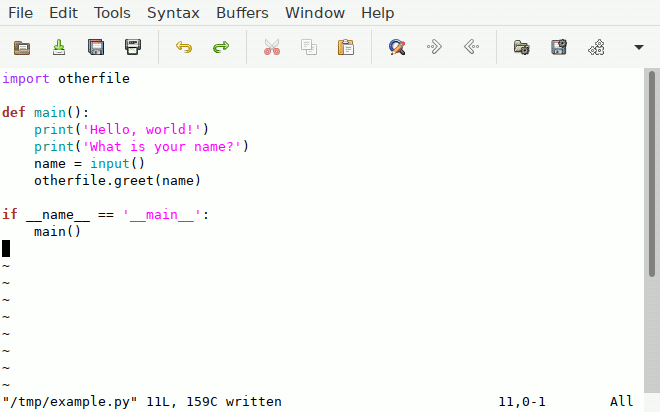
\includegraphics[width=0.9\textwidth]{fig/editor}
            \begin{itemize}
                \item Write code in editor (e.g., Sublime Text, Notepad++, Vim)
                \item Save as plain text in .py files
                \item import functions from other .py files
            \end{itemize}
        \pause
        \column{0.5\linewidth}
            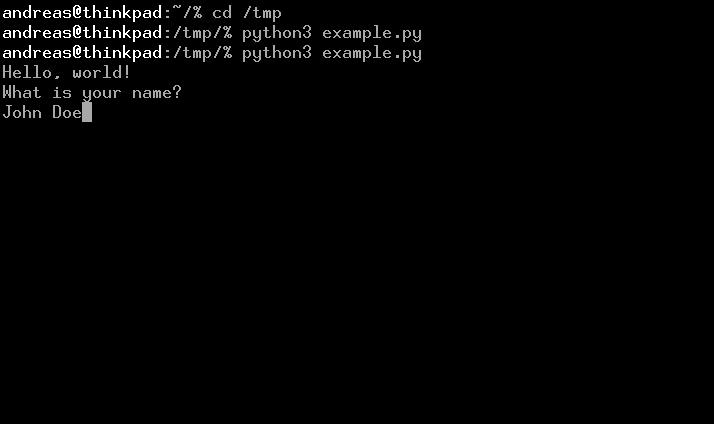
\includegraphics[width=0.9\textwidth]{fig/terminal}
            \begin{itemize}
                \item Run code in a terminal
            \end{itemize}
    \end{columns}
\end{frame}

\begin{frame}{Learn more}
    Recommended further materials:
    \vspace{1em}
    \begin{itemize}
        \item \url{https://jakevdp.github.io/PythonDataScienceHandbook/}
        \item \url{https://ProgrammingHistorian.org/en/lessons/}
        \item \url{https://AutomateTheBoringStuff.com/}
    \end{itemize}
\end{frame}

\begin{frame}\Huge\centering
    That's all, folks!
\end{frame}

\begin{frame}
Materials used for these slides:
\begin{itemize}
\item \url{https://www.cs.umd.edu/class/fall2018/cmsc320/}
    specifically lecture 11
    % https://www.cs.umd.edu/class/fall2018/cmsc320/lecs/cmsc320_f2018_lec11.pdf
\item \url{https://mlcourse.ai/}
    specifically lecture 1
\end{itemize}

\vspace{1em}
Documentation:
\begin{itemize}
    \item \url{https://pandas.pydata.org/pandas-docs/stable/}
    \item \url{https://pandas.pydata.org/pandas-docs/stable/getting_started/comparison/comparison_with_sql.html}
    \item \url{https://seaborn.pydata.org/tutorial.html}
\end{itemize}
\end{frame}

\end{document}
